\section{Applications}

This section explores the potential of the proposed method in practical applications, with a focus on analyzing its advantages over traditional techniques in terms of deployment convenience, adaptability to complex shapes, and support for emergent gameplay design.

\subsection{Easy Deployment in Real Time Applications}

In real-world project development, some engineering practices may adopt a naive buoyancy estimation based solely on the center-of-mass position to minimize implementation complexity. Although computationally inexpensive, such methods often result in unnatural rotational postures during floating or sinking processes. As shown in Figure \ref{fig:bad-donut}, a lifebuoy may tilt unrealistically while floating on the water surface, severely affecting immersion.

\begin{figure}[H]
	\centering
	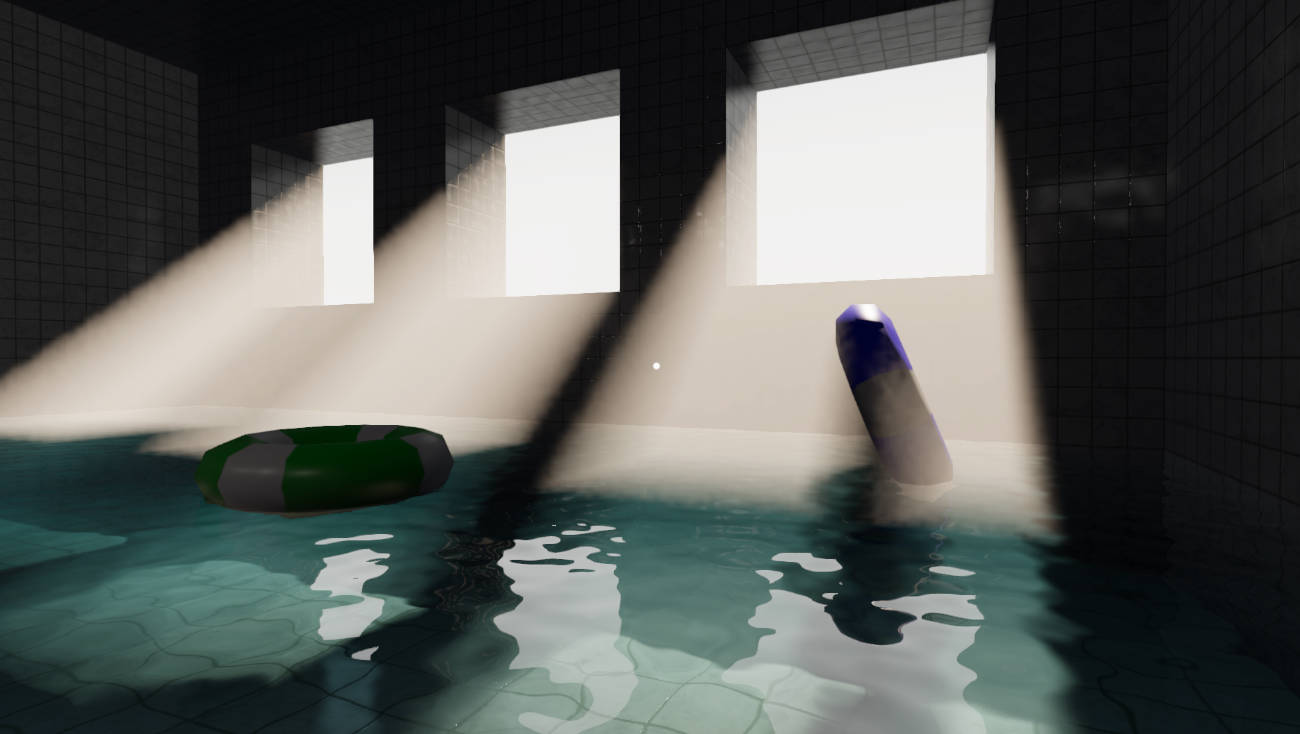
\includegraphics[width=0.5\textwidth]{./figures/bad-donut.jpg}
	\caption{A lifebuoy floating at an awkward angle.}
	\label{fig:bad-donut}
\end{figure}

To address this issue under real-time constraints, the traditional solution is to configure sphere pontoons for each floating object, simulating localized buoyancy distribution. While carefully tuned configurations can yield good results, the manual workload rapidly escalates with the diversity and quantity of objects, and human error becomes increasingly likely.

The proposed Monte Carlo surface sampling method eliminates the need for manual proxy setup. Once an object is equipped with the system, buoyancy forces and torques are estimated in real time under full system management. This greatly simplifies both development and asset production workflows, making the method particularly suitable for projects involving a wide variety of objects and frequent dynamic changes.

\subsection{Realism on Complex Objects}

For objects with complex shapes, especially those with extreme aspect ratios, manual sphere pontoon configurations inherently struggle to capture the realistic geometrical characteristics. If the density of proxy points is insufficient, floating and rotational behaviors may appear unnatural.

Our method estimates buoyancy based on true physical surface forces and theoretically adapts to arbitrary complex geometries without requiring special attention to the geometrical features. This ensures consistent and physically plausible behavior even for highly detailed models.

\subsection{Emergent Gameplay Design}

Because it requires no manual configuration and can adapt to complex geometries in real time, the proposed method enables game designers to freely integrate buoyancy mechanisms into various gameplay systems. For instance, players can stack existing floating objects to build bridges, create makeshift pontoons, construct floating platforms, or manipulate object center of mass and posture to achieve specific objectives.

As illustrated in Figure \ref{fig:boat-sample}, using our method, a boat's draft depth dynamically changes with the weight of loaded cargo without the need for additional setup. This low-barrier, high-flexibility design space significantly enhances emergent behavior, providing developers with richer opportunities for dynamic content generation and interactive gameplay.

\begin{figure}[H]
	\centering
	\begin{subcaptionblock}{0.46\textwidth}
		\centering
		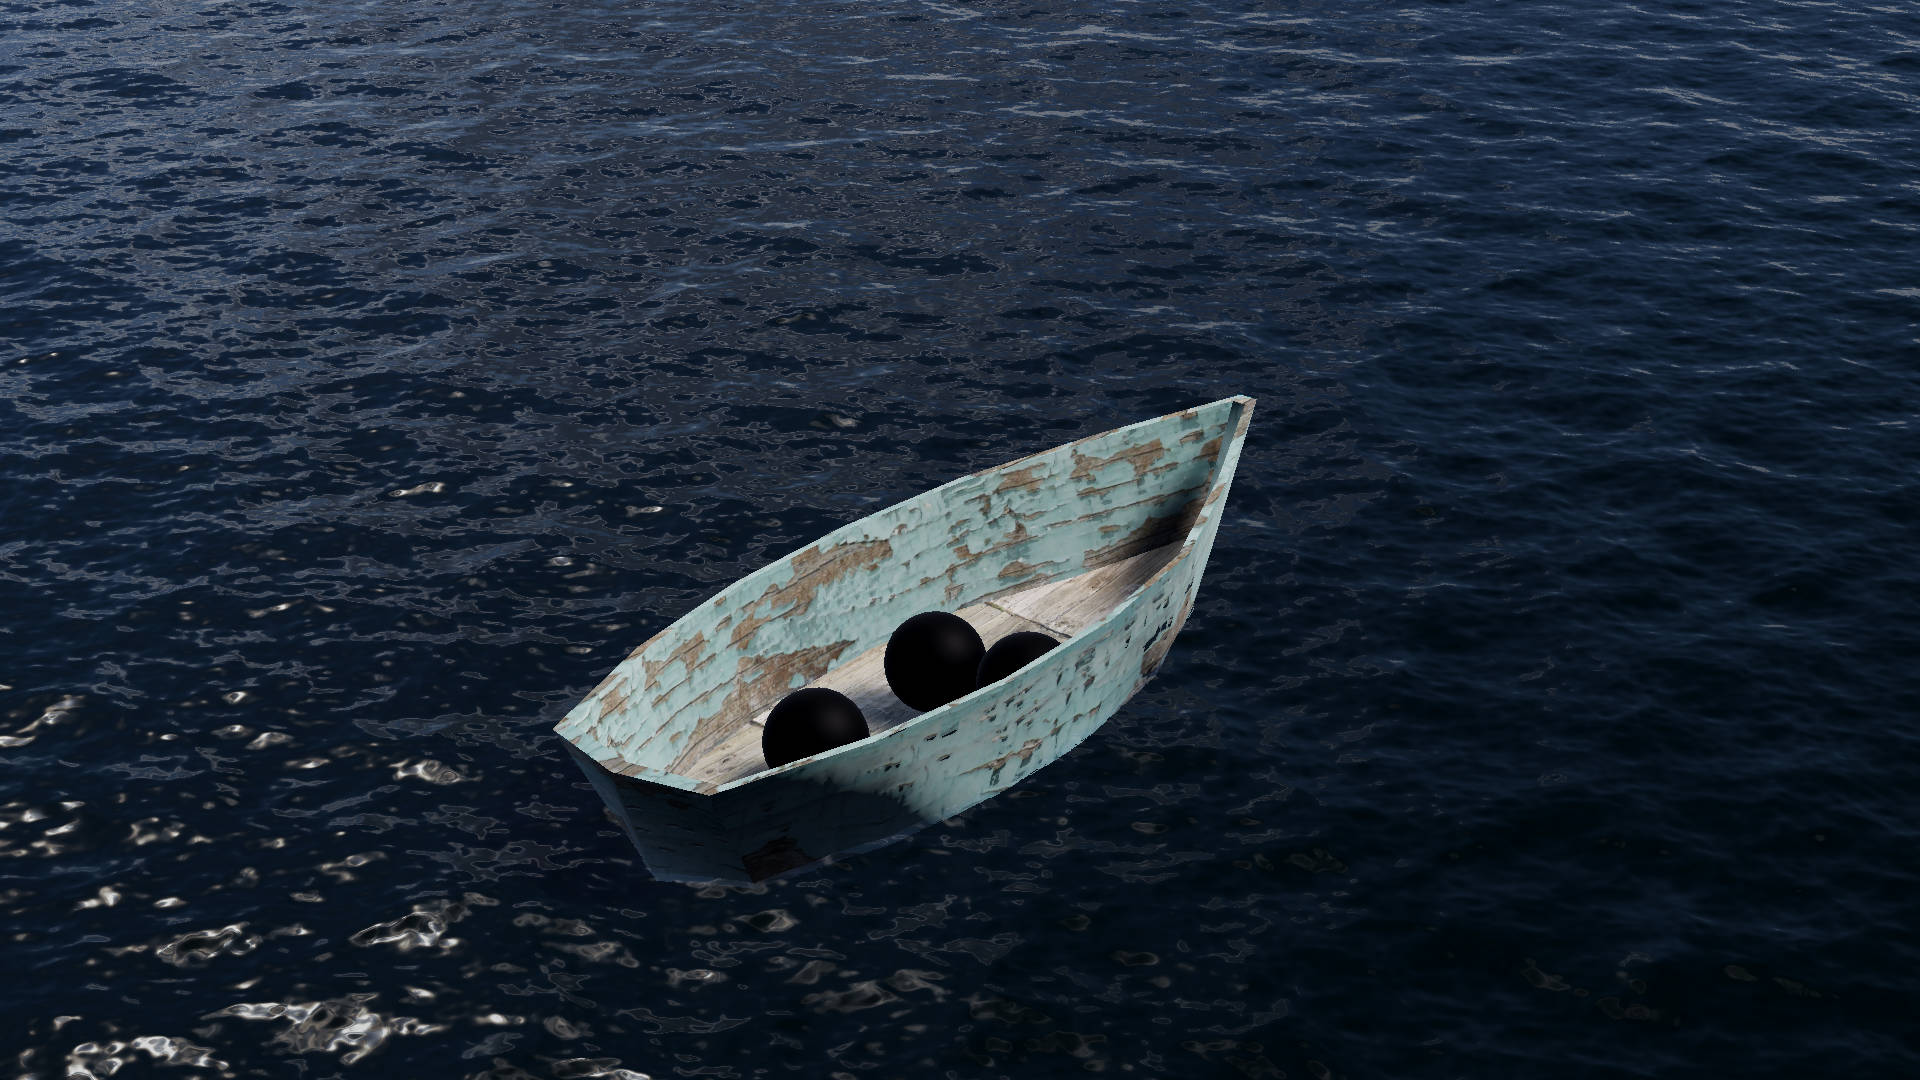
\includegraphics[width=0.9\textwidth]{../Thesis/figures/light-boat.jpg}
		\caption{A boat containing a few balls.}
	\end{subcaptionblock}
	\begin{subcaptionblock}{0.46\textwidth}
		\centering
		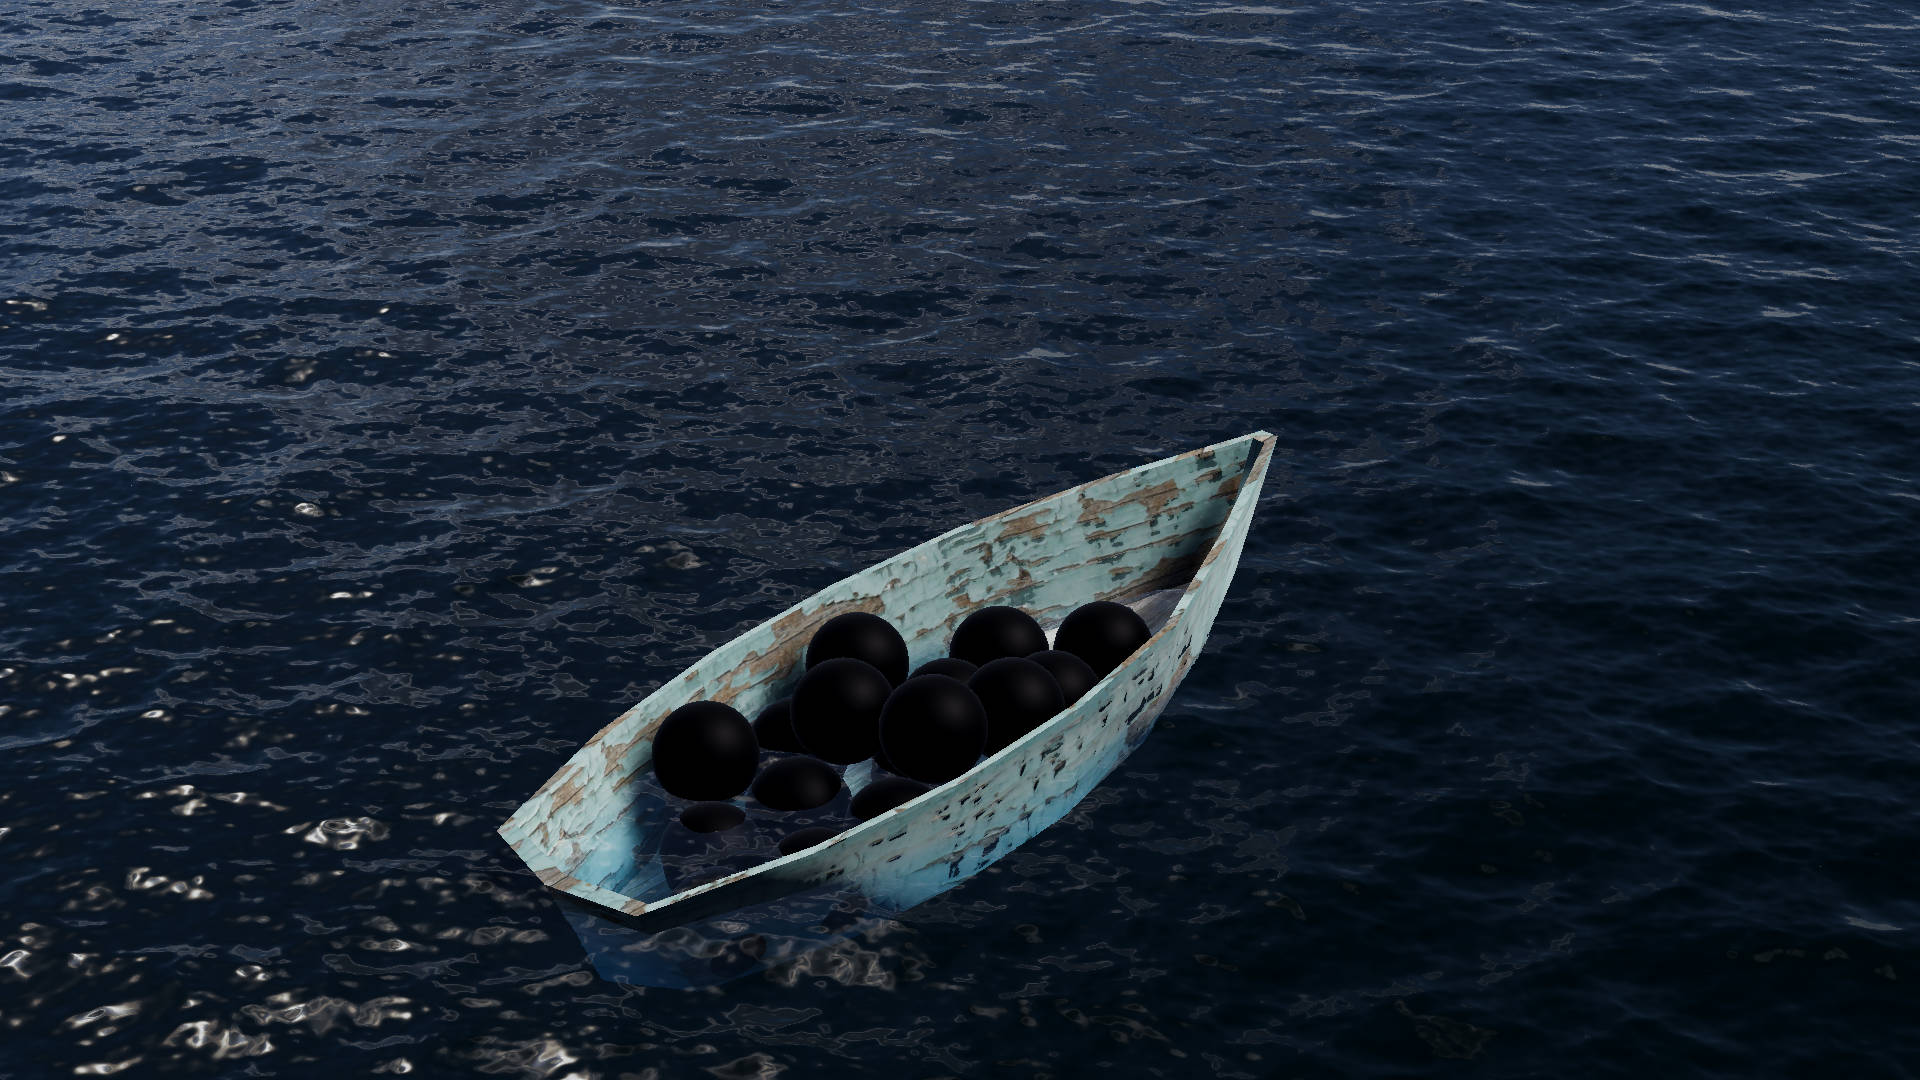
\includegraphics[width=0.9\textwidth]{../Thesis/figures/heavy-boat.jpg}
		\caption{The same boat containing many balls.}
	\end{subcaptionblock}
	\caption{Loading more balls onto the boat increases its depth.}
	\label{fig:boat-sample}
\end{figure}


\begin{comment}
Figure \ref{boat-sample} shows a basic usage case of our method.
A boat is floating on the sea; a pack of heavy balls are spawning above the boat and falling into it.
Without having to write any additional codes, just by keeping loading heavy balls onto the boat, the sunk depth of the boat automatically increases.

\begin{figure}[H]
	\centering
	\begin{subcaptionblock}{0.46\textwidth}
		\centering
		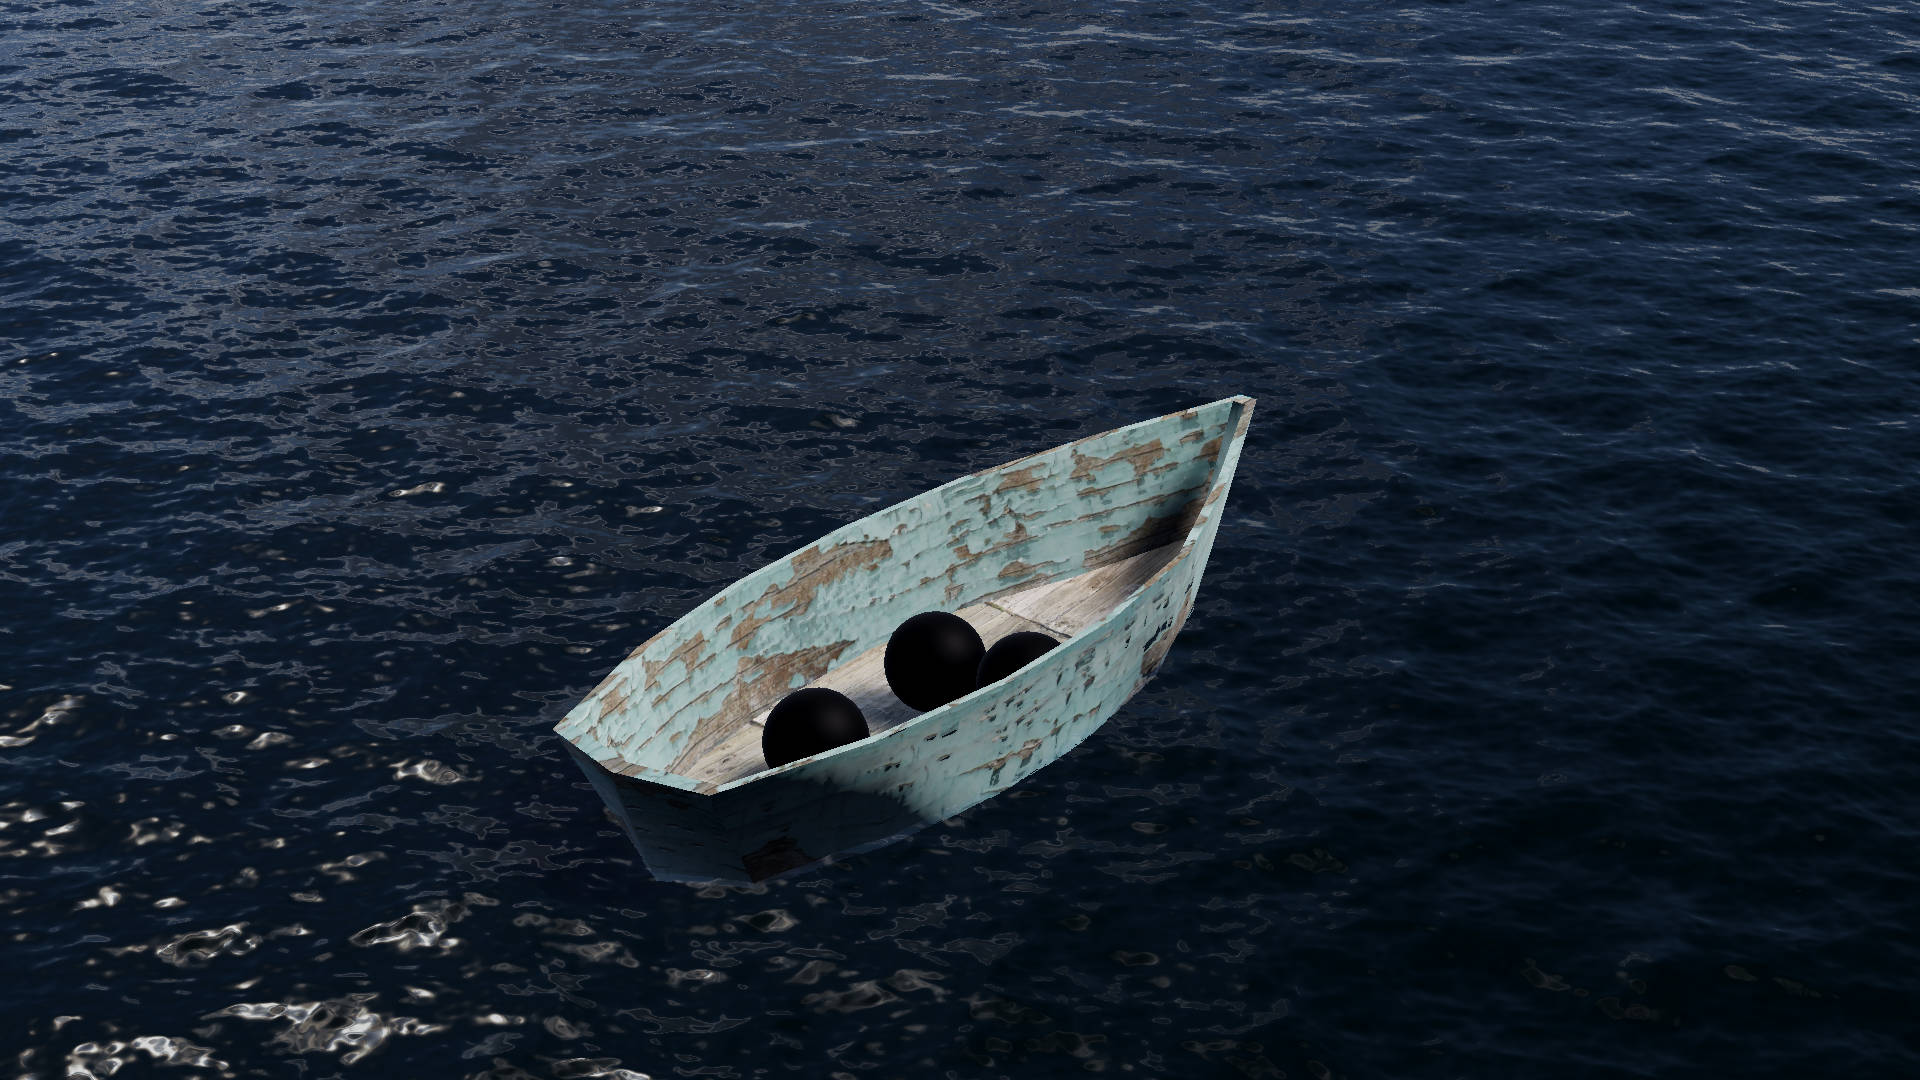
\includegraphics[width=0.9\textwidth]{../Thesis/figures/light-boat.jpg}
		\caption{A boat containing a few balls.}
	\end{subcaptionblock}
	\begin{subcaptionblock}{0.46\textwidth}
		\centering
		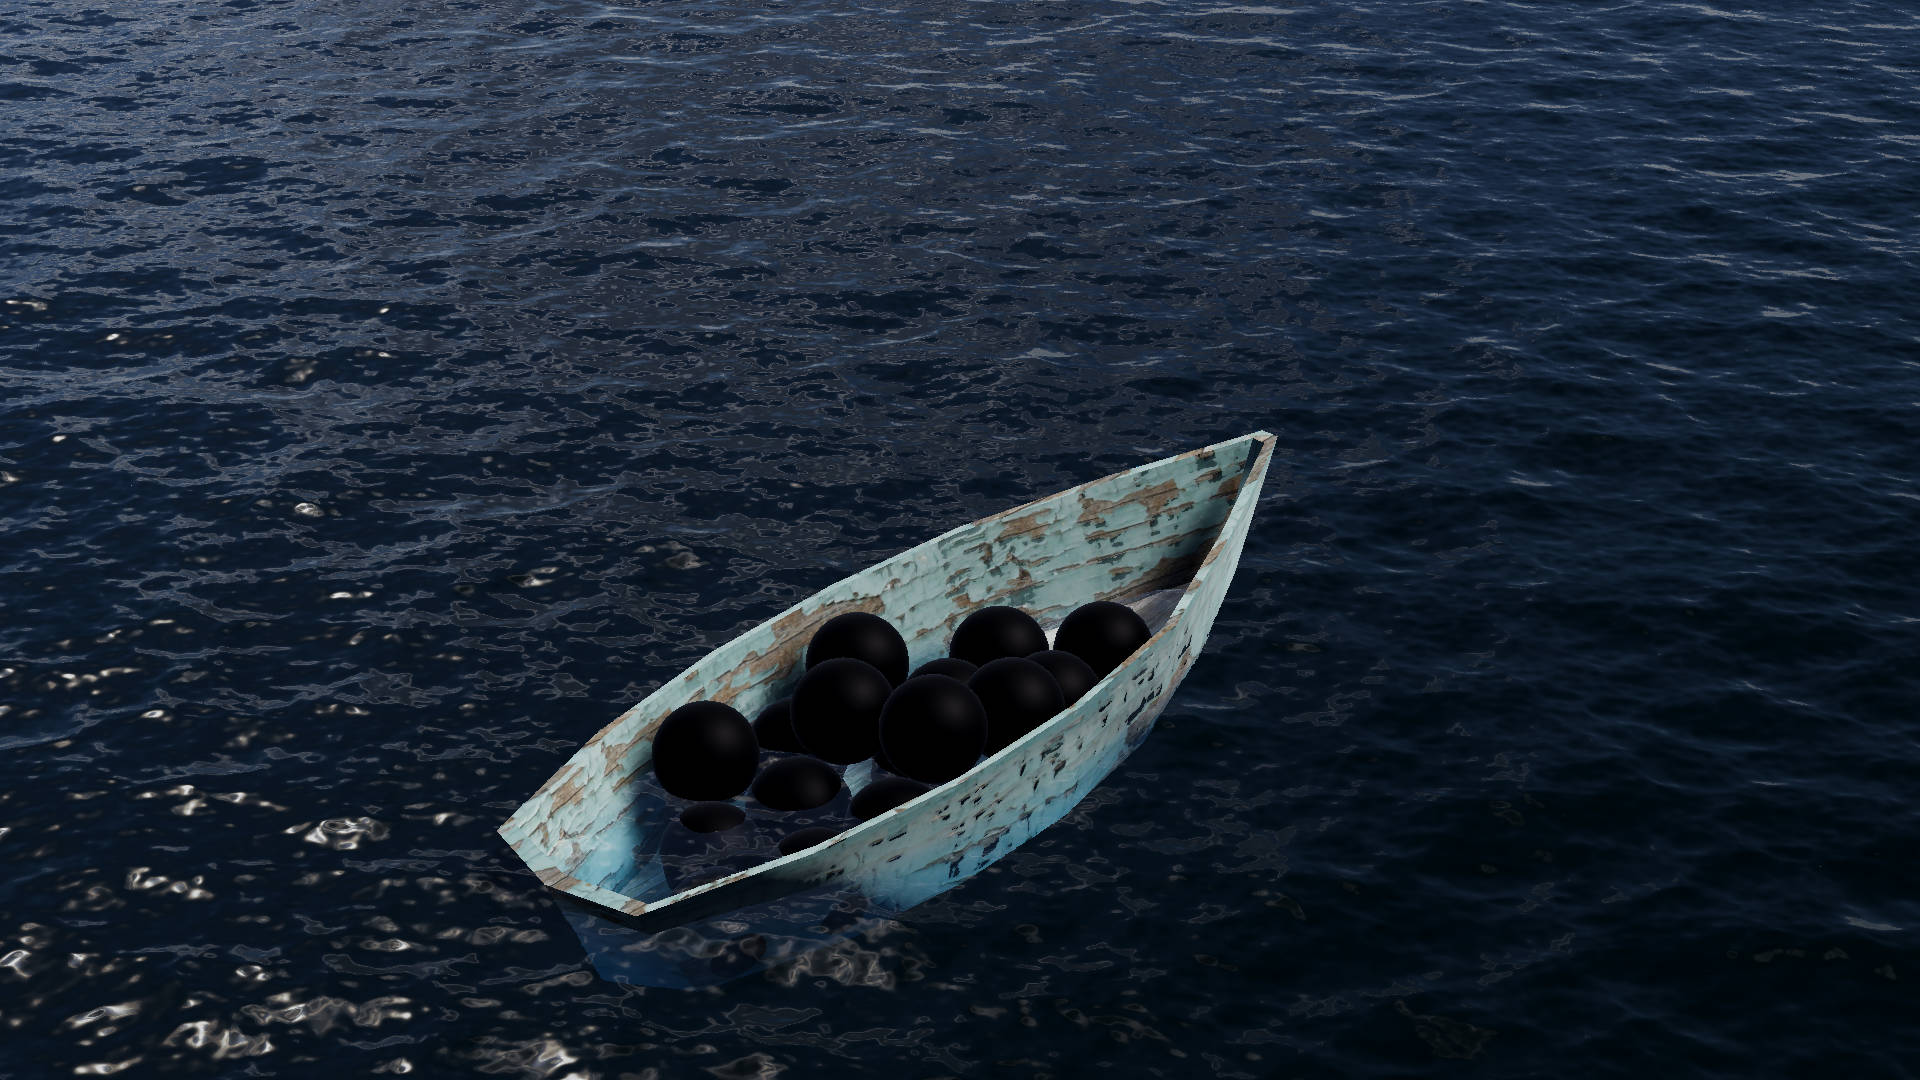
\includegraphics[width=0.9\textwidth]{../Thesis/figures/heavy-boat.jpg}
		\caption{The same boat containing many balls.}
	\end{subcaptionblock}
	\caption{Loading more balls onto the boat increases its depth.}
	\label{boat-sample}
\end{figure}

When applied in real game design, this extra freedom could allow game designers to create more complex mechanisms.
It is clear that often an open mechanism tends to lead to emergent behaviors \cite{sweetser2006emergent}, thus increasing the fun of the game.

Buoyancy simulation could also be used for creating the vibes.
Figure \ref{floating-donut-in-game} shows a screenshot of a poolcore-themed puzzle game, in which water is a main part of the visual design.
Adding objects that could float on water definitely helps emphasize the vibes of the pools.

\begin{figure}[H]
	\centering
	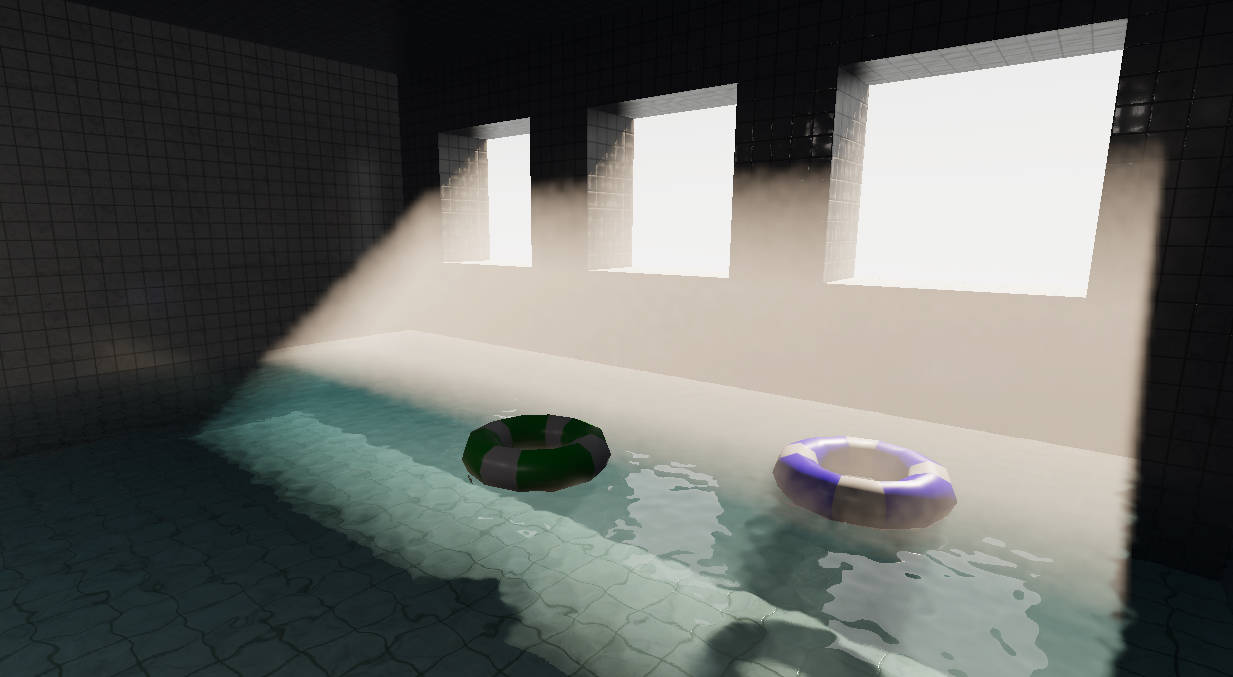
\includegraphics[width=0.4\textwidth]{../Thesis/figures/floating-donut-in-game.jpg}
	\caption{Floating objects can be seen in a poolcore-themed game.}
	\label{floating-donut-in-game}
\end{figure}
\end{comment}